\begin{frame}{Dynamics}  %% ---------- Intro/motivation 
    \begin{tikzpicture}[overlay,remember picture]
        \uncover<1->{ % <-> |
            \node (t1) [anchor=center,scale=1,opacity=1] at ([shift={(-0.6cm,-0.0cm)}]current page.center){
                \parbox{1.\textwidth}{
                    Semi-analytic model (energy conservation) in a 
                    thin-shell  approximation:\\%\footcite{Nava:2013,Kumar:2014upa,Zhang:2018book}; \\
                    
                    %From stress-energy tensor %$ T^{\mu\nu} = (\rho' c^2 + p') u^{\mu}u^{\nu} + p' g^{\mu\nu}$ \\
                    %we write evolution equation: 
                    \vspace{-2mm}
                    \begin{equation*}
                        \begin{aligned}
                            dE_{\rm tot} = 0 \rightarrow & d [ \Gamma (M_0 + m) c^2 + \Gamma_{\rm eff}E_{\rm int}' ] = dm c^2 + \Gamma_{\rm eff} dE_{\rm rad}'. \\
                            & dE_{\rm int}' = dE_{\rm sh}' + dE_{\rm ad}' + dE_{\rm rad}',
                        \end{aligned}
                    \end{equation*}
                    
                    Adiabatic evolution, $\Gamma=f(R)$; \\
                    If $\rho_{\rm ISM}=\text{const}$: free-coasting ($\Gamma=\Gamma_0$), and deceleration,  $\Gamma\downarrow$.\\
                    
                    \textbf{Structure:} lateral, $\{\theta_i\}$, and velocity $\{\upsilon_i\}$; \\
                    \textbf{Initial conditions}: ejecta profile, \\
                    $\{ E_{ij, 0} \}=f(\Gamma_{i, 0},\theta_{j, 0})$. %($\Gamma=(1-\beta^2)^{-2}$); $\beta=\upsilon/c$; \\
                    %\textbf{Main stages:} free-coasting + deceleration; \\
                    %$\Gamma$ is the bulk Lorentz factor. \\
                    %\textbf{Shock properties}, $\rho_{\rm sh}$, $\beta_{\rm sh}$, $R_{\rm sh}$ \\
            }};
            
        }
        %        \uncover<1->{ % <-> |
            %            \node (t1) [anchor=center,scale=1,opacity=1] at ([shift={(4.0cm,-2.0cm)}]current page.center){
                %                \parbox{0.5\textwidth}{
                    %                    \textbf{Evolution}: free-coasting + deceleration; \\
                    %                    %Electrons accelerated to power-law distribution $\gamma_e^{-p}$
                    %                    Total energy in electrons and magnetic fields $\epsilon_e$, $\epsilon_B$;
                    %                    Assume for electrons local istropic distribution of angles relative $\vec{B}$; \\
                    %                    Assume $\vec{B}$ is random mix of orientations; \\
                    %                    Spectrum from a PL electrons is also PL; \\
                    %                    %Assume local cooling rate $=$ expansion time
                    %                    Emission is isotropic in the rest-frame
                    %                    %Intensity-weighted mean change in any charactersitic gets broadened
                    %            }};
            %        }
        % Margalit B., Quataert E., 2021, ApJL, 923, L14. 
        %        \uncover<1->{ % <-> |
            %            \node (t1) [anchor=center,scale=1,opacity=1] at ([shift={(-4.4cm,-2.4cm)}]current page.center){
                %                \parbox{0.5\textwidth}{
                    %                    \begin{equation*}
                        %                        P_{\nu'} = \int_{\gamma_{\nu'}}^{\infty} d\gamma_e \frac{dn'}{d\gamma_e}P_{s}'(\nu'); \hspace{3mm} \frac{dn'}{d\gamma_e} \propto
                        %                        \begin{cases}
                            %                            \gamma_e^{-2} &\text{s.c.} \\ 
                            %                            \gamma_e^{-p-1} &\text{f.c.}
                            %                        \end{cases}
                        %                    \end{equation*}
                    %                    %
                    %                    \begin{equation*}
                        %                        F(\nu,t) = \frac{1+z} {2d_L^2}\int_0^{\theta}\int_{0}^{r}\frac{P'(\nu',t_{\rm em},r)}{\Gamma^2(1-\beta\cos\theta)^2}r^2 dr d\cos\theta
                        %                    \end{equation*}
                    %                    \textbf{Synchrotron Radiation}
                    %            }};
            %        }
        
        %        \uncover<1-1>{ % <-> |
            %            \node (img1) [anchor=center,scale=1,opacity=1] at ([shift={(4.5cm,-0.3cm)}]current page.center){
                %                \parbox{0.6\textwidth}{
                    %                    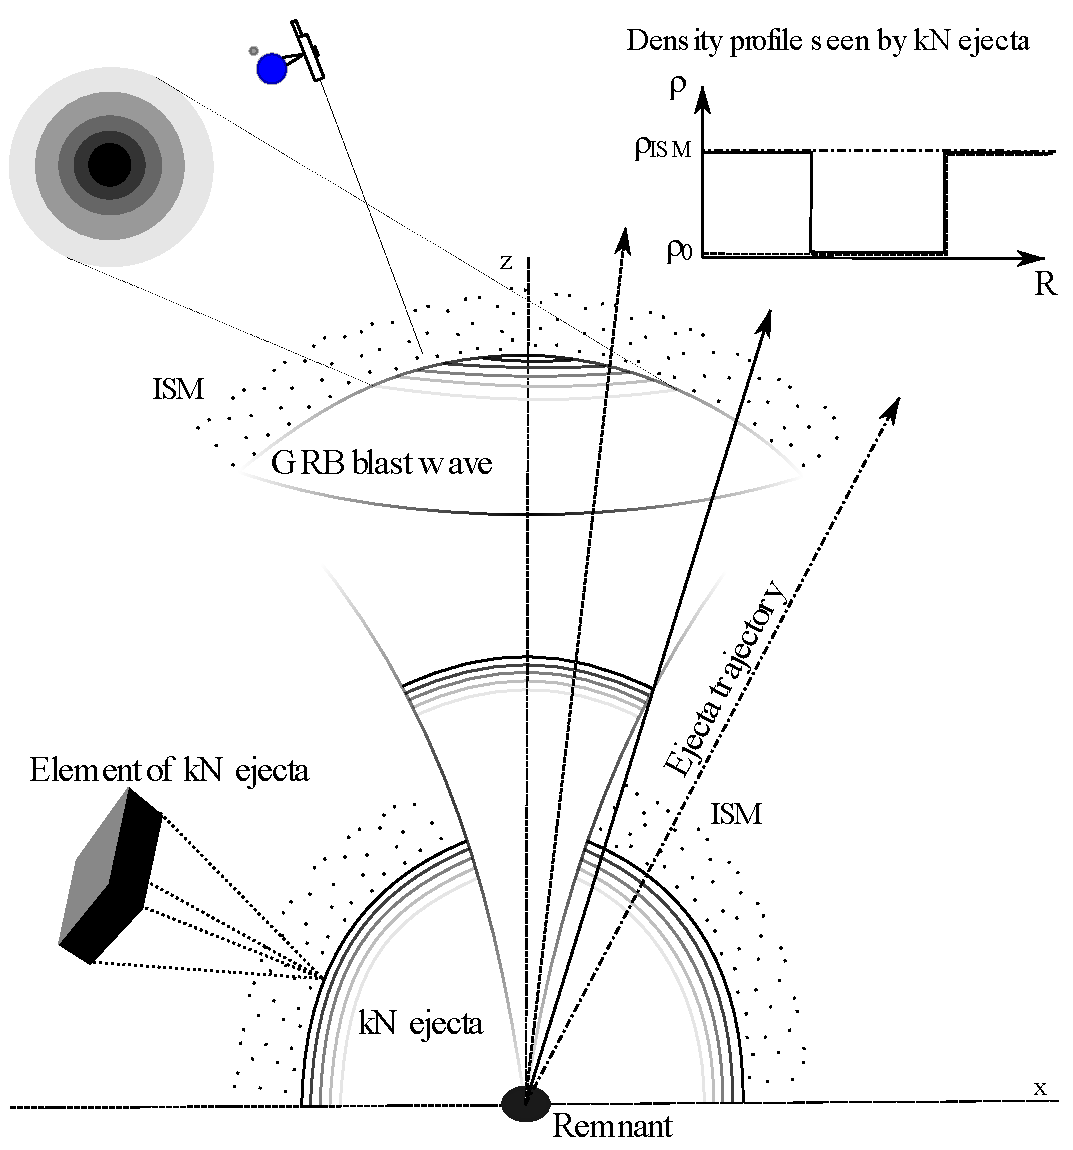
\includegraphics[height=7.8cm]{figures/structure2.pdf}
                    %                    %\includesvg[height=7.2cm]{figures/structure2}
                    %            }};
            %        }
        \uncover<1->{ % <-> |
            \node (img1) [anchor=center,scale=1,opacity=1] at ([shift={(5.0cm,-2.4cm)}]current page.center){
                \parbox{0.6\textwidth}{
                    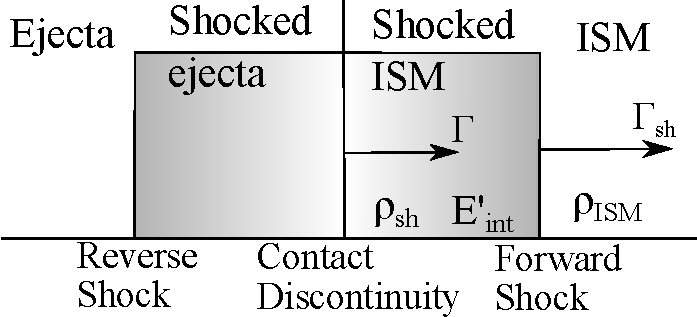
\includegraphics[height=3.0cm]{../figs/shock_scatch2.pdf}
            }};
            
        }
        
    \end{tikzpicture}
\end{frame}


\begin{frame}{Radiation}  %% ---------- Intro/motivation 
    \begin{tikzpicture}[overlay,remember picture]
        \uncover<1->{ % <-> |
            \node (t1) [anchor=center,scale=1,opacity=1] at ([shift={(-3.6cm,1.4cm)}]current page.center){
                \parbox{0.6\textwidth}{
                    \textbf{A shock}:\\%\footcite{Zhang:2018book}:%$^{\textcolor{gray}{\text{\cite{Rezzolla:2013,Kumar:2014upa,Zhang:2018book,Nava:2013}}}}$
                    \begin{itemize}
                        \item compresses fluid, $\rho_{\rm sh} = 4; \Gamma_{\rm sh} \rho_{\rm ISM}$;
                        \item amplifies magnetic fields, $B=\sqrt{8 \pi \epsilon_B e'}$;
                        \item accelerates electrons, $\frac{dn'}{d\gamma_e} \propto \gamma_e^{-p}$.
                    \end{itemize}
                    
            }};
            
        }
        \uncover<1->{ % <-> |
            \node (t1) [anchor=center,scale=1,opacity=1] at ([shift={(4.6cm,1.3cm)}]current page.center){
                \parbox{0.6\textwidth}{
                    \textbf{Synchrotron radiation spectrum} \\%$^{\textcolor{gray}{\text{\cite{Sari:1997qe}}}}$ \\
                    Broken power law (BPL)\\%\footcite{Sari:1997qe,Wijers:1998st}; \\ 
                    %$\nu_m\propto\gamma_m$, $\nu_c\propto\gamma_c$ \\
            }};
            
        }
        
        %        \uncover<1->{ % <-> |
            %            \node (t1) [anchor=center,scale=1,opacity=1] at ([shift={(-4.4cm,-1.7cm)}]current page.center){
                %                \parbox{0.5\textwidth}{
                    %                    \textbf{Electron spectrum}: %$^{\textcolor{gray}{\text{\cite{Sari:1997qe}}}}$ \\
                    %                    broken power law (BPL) with 
                    %                    \vspace{-3mm}
                    %                    \begin{equation*}\label{eq:method:gm_pl_only}
                        %                        \gamma_m' = \frac{p-2}{p-1} \frac{\epsilon_e e'}{n' m_e c^2} \hspace{3mm} 
                        %                        \gamma_c' = \frac{6 \pi m_e c \Gamma}{\sigma_T t_{\rm em} B'^2}, \hspace{3mm}
                        %                        %e' = \frac{E_{\rm int}'}{V'}
                        %                    \end{equation*}
                    %                \vspace{-5mm}
                    %                    \begin{footnotesize}
                        %                        \begin{itemize}
                            %                            \item Slow cooling $\gamma_m' < \gamma_c'$
                            %                            \item Fast cooling $\gamma_m' > \gamma_c'$
                            %                        \end{itemize}
                        %                    \end{footnotesize}
                    %            }};
            %        }
        \uncover<1->{ % <-> |
            \node (t1) [anchor=center,scale=1,opacity=1] at ([shift={(-4.4cm,-1.5cm)}]current page.center){
                \parbox{0.5\textwidth}{
                    \textbf{Spectral breaks}: 
                    \begin{itemize}
                        \item $\nu_m$ -- injection break; %at which most of the injected electrons radiate 
                        \item $\nu_c$ -- cooling break; %at which for electrons expansion timescale is equal to the radiative cooling timesacle
                        \item $\nu_a$ -- absorption break. % below which synchrotron emission is absorbed by electrons in free-free transitions in magnetic
                    \end{itemize}
                    \vspace{4mm}
                    \textbf{EATS} integration $\rightarrow$ $F_{\nu}(t_{\rm obs})$
            }};
        }
        
        
        \uncover<1->{ % <-> |
            \node (img1) [anchor=center,scale=1,opacity=1] at ([shift={(3.6cm,-1.6cm)}]current page.center){
                \parbox{0.6\textwidth}{
                    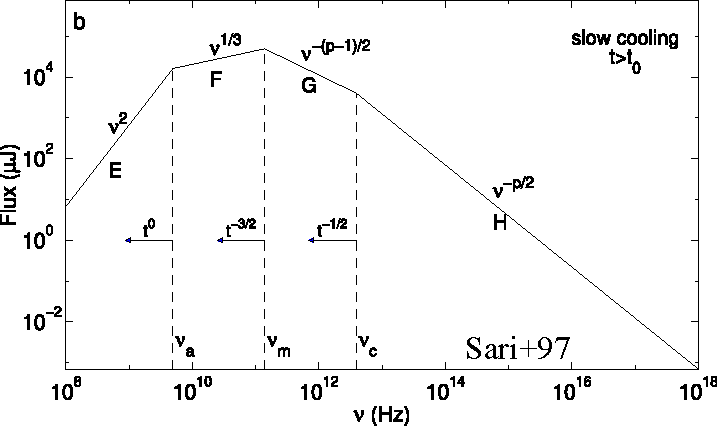
\includegraphics[height=5.0cm]{../figs/Sari97_spectrum_slow_cool.pdf}
                    %                        Overall, an afterglow spectrum has three characteristic frequencies: 
                    %                        (i) $\nu_i$ (injection break) at which most of the injected electrons radiate 
                    %                        (ii) $\nu_c$ (cooling break) at which for electrons expansion timescale is equal 
                    %                        to the radiative cooling timesacle
                    %                        (iii) $\nu_a$ an absorption break, below which synchrotron emission is absorbed by 
                    %                        electrons in free-free transitions in magnetic fields, (\ac{SSA}).
            }};
        }
    \end{tikzpicture}
\end{frame}

\begin{frame}%{Representative picture of a binary neutron star merger} %% ---------- title 
    \begin{tikzpicture}[overlay,remember picture]
        \uncover<1->{ % <-> |
            \node (t1) [anchor=center,scale=1,opacity=1] at ([shift={(-4.1cm,-2.1cm)}]current page.center){
                \parbox{0.50\textwidth}{
                    % Grav. radiation losses cause the orbital separation to shrink (Softer EOSs -- longer inspiral)
                    % Inspiral (${\simeq}10\,$orbits); NSs Zero-temperature, $\beta$-equilibrium \\
                    % Merger \& post-merger, $T{\sim}50\,$MeV, $\rho{\sim3.6}\rho_0$. \\
                    % Postmerger: Remnant $+$ disk $+$ ejecta; \\
                    % Fate: $J$ transport; MHD; $\nu$, GWs \\
                    \textbf{Key parameters:} \\
                    tidal interaction 
                    % Distrortion of the mass distribution of a given NS in a Grav. Field of another
                    % Parametrized with Love Number (computed by solving perturbation of a relativistic star k=f(EOS,Compactness))
                    % Combining compactness and Love we get tidal polarizability parameter
                    % The dynamics of the two bodies can be described with tidal coupling constant that 
                    % describes tidal interaction at leading order
                    % Tidal interaction (i) attractive (ii) short range: They accelerate merger, increase frequency
                    can be parameterized with \textit{reduced tidal parameter}%\footcite{Favata:2013rwa}%$^{\text{\textcolor{gray}{\cite{Favata:2013rwa}}}}$
                    %
                    \begin{equation*}
                        \tilde{\Lambda} := \frac{16}{13}\frac{(M_A + 12M_B)M_A^4 \Lambda_A}{M^5}+(A\leftrightarrow B).
                    \end{equation*}
                    % Gravitational massess are estimated in (conformal, assymptitic? flatness?) in far-field regime and are estimated as integrals over fluid configuration
                    %
                    $\downarrow\tilde{\Lambda}$ for softer EOS, $\uparrow M$, $\uparrow q=M_A/M_B$ \\
                    %
                    % A moment of merger is a maximum of the GW amplitude
                    %
                    % Gauge invariant quantities: Reduced binding energy and angular momentum
                    % During the evolution they decrease as GW carry energy away
                    % Quasiuniversality: EOS can be captured with $\tilde{\Lambda}$ for equal mass binary
                    % 
                    % 
            }};
        }
        %
        \uncover<1->{ % <-> |
            \node (t1) [anchor=center,scale=1,opacity=1] at ([shift={(4.2cm,-2.0cm)}]current page.center){
                \parbox{0.55\textwidth}{
                    \textbf{Ejecta}:
                    \begin{itemize}
                        \item dynamical (${\lesssim}10\,$ms),
                        \item secular (${\gtrsim 10\,}$ms).
                    \end{itemize}
                    \vspace{5mm}
                    \textbf{Post-merger state:} \\
                    BH or long/short-lived remnants \& disks. \\
                    % Early postmerger: 
                    % Core bounces: cold cores, hot interface; shocks at NS surface only \\
                    % Right after the merger double-core structure is formed by the two central cores of merging NSs. Cors collide and bounce repeadetly untill they merge. In this process outer layers gain J due to Orbital Angular Momentum Advection and Torques arasing from double-core, non-axisymmetric structure of the sustem. Result: core immersed in low-rho cloud
                    % Neutrino burst, ${\sim}15\,$MeV. 
                    % Neutrino decouple at different radii
                    % Abundance of free $n$, absorbe $\nu_e$, raise $Y_e$; emission of $\bar{\nu}_e$
                    % Possible phase transition softens EOS
                    % Impact of phase transition depends on density at which it occure
                    % While cores fuse, remnant is \textit{deformed} \\%remnant shows bar-like deformation \\
                    % Main post-merger GW freq. = 2 times dynamical freq.
                    % Peaks in GWs associated with hydro mode 
                    % Peak frequencies depend on NS prop. -- quasiuniversality
                    % Ang. Mom. at merger determines the angular vel. of the bulk of matter
                    % Most luminous $\neq$ largest energy
                    % Simulations give upper limitof GWs energy
                    % GWs backreacts on the fluid, damping the non-axisymmetric modes
                    % Remnant evolves towards \textit{axisymmetry} \\
                    % Postmerger state: super-Keplerian $J>J_{\rm max}^{\rm equilib}$, $M_b>M_{b \rm, max}^{\rm eqilib}$ -- Highly differential rotation remnant
                    % Thermal and neutrino effects $\uparrow$ pressure (${\simeq}10\%$), hence, radius, but not the $M_{\rm max}$. 
                    % Rotatin increases NS $M_{\rm max}$ and $R$. 
                    % Note: In postmerger $M_{\rm max}^{\rm hot} < M_{\rm max}^{\rm cold}$
                    % hence, temperature effects do not stabilize the star.
                    % Larger radiuss $\rightarrow$ lower mass-shedding limit
                    % Overall: cold classification do not (SMNS, HMNS...) do not apply
                    % Magnetic fields can raise $M_{\rm max}$, affecting angular momentum distribution
                    % Angular momentum redistribution occures on a viscous time-scale.
                    % Inclusion of viscosity show shorter collapse time. 
                    % Simulations show a ritational profile with a minimum at the core; as viscous and hydro effects counteract Grav. instabilities in the core, the core will spin up, compactness reduces, hence, the core must shed the excess in angular momentum. Through winds!
                    % Neutrinos primarely cool the remnant, removing some of the excess in binding energy. 
                    % Simulations show that one-armed instability persists on ${\sim}50\,$ms timescale.
                    % Disk $\rho < 10^{13}\,$\gcm
                    % Volume integral of the conserved rest-mass density
                    % Properties depend on formation
                    % formed from matter expelled by tidal torquies at merger 
                    % Structure: coled tidal component $+$ hot shocked
                    % Nass of the disk may rise as $M_b$ and $J$ are shed by the remnant
                    % Shocks ($m=1$) raise entropy, Keplerian, temp profile $\{10,0.1\}$MeV
                    % BH formation removes ${\sim}50$ disk
                    % Disks around BHs are more compact and hotter
                    % In case of PC, $q=1$ binaries give little disk, while $q{\simeq}1.4$ result in more massive disks. Hiher $q$ lead to tidal disruption of a compantion and formation of a massive cold disk.
                    % In high $q$ cases tidal tail falls back, disturbing the disk
                    % -------
                    % Constraints on NS mass and radius can come from NICER, XMM, NANOGrav, of pulsars and LVC of GW170817
                    % Disk formation After merger, anguilar momentum is transfered from inner to the outer layers causing outer layers to expand (and it will remain outside the ISCO when BH forms). 
                    % In prompt collapse cases the disk expected to be smaller as there is no angular momentum transport due to turbulence. Only external and low density outer layers of the star are able to gaun enough angular momentum die to tidal torques and pushed away from the bulk of the merging stars. 
                    % Soft EOS remnant cannot hold high J by tidal torques. 
            }};
        }
        
        \uncover<1->{ % <-> |
            \node (img1) [anchor=center,scale=1,opacity=1] at ([shift={(-1.cm,1.8cm)}]current page.center){
                \parbox{1.0\textwidth}{
                    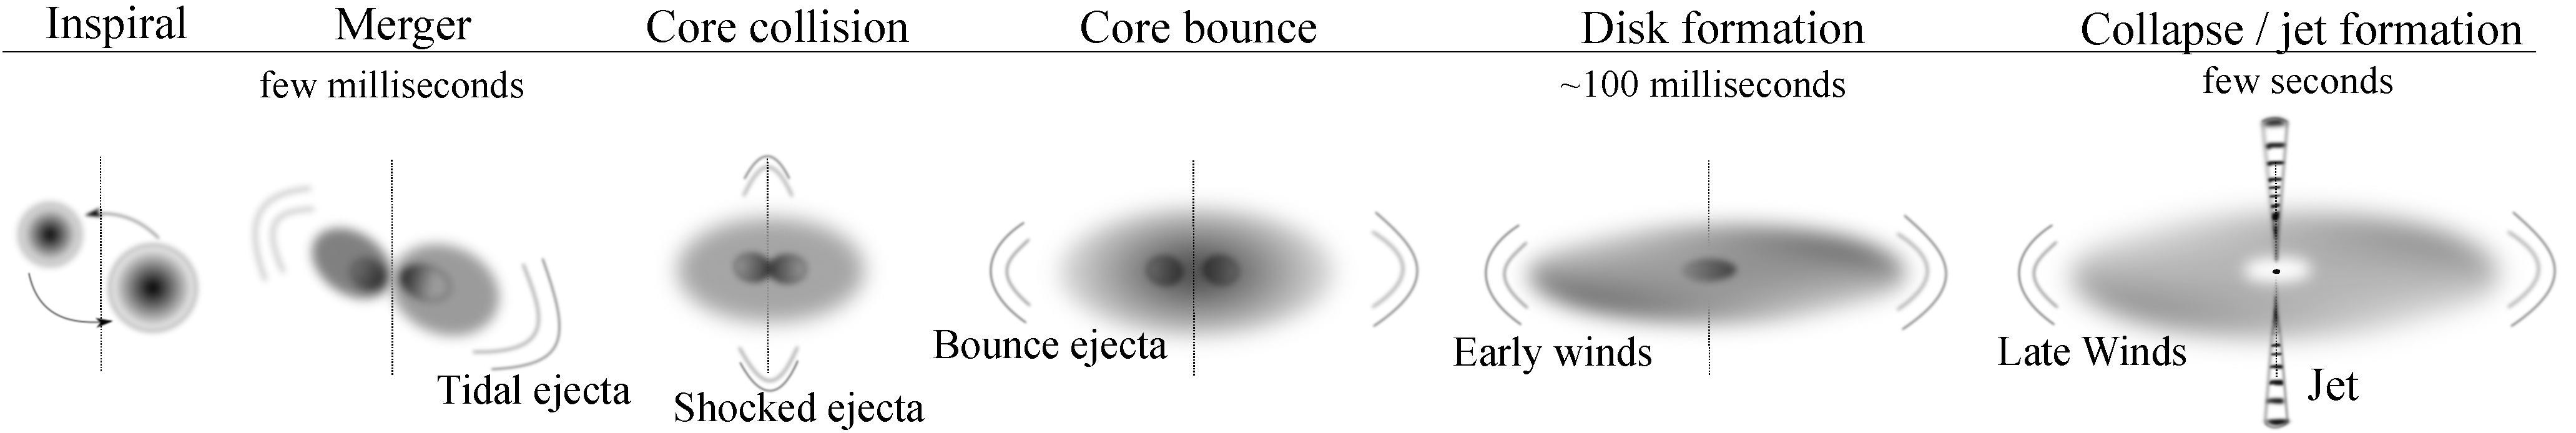
\includegraphics[height=2.7cm]{../figs/bns_evolution_transparent.pdf}
                    %            \hspace*{10mm} Density modes in the remnant 
                    %Modes analysis for exemplary equal-mass long-live and short-lived
                    %        remnants. The evolution of the $m=2$ and the $m=1$ monitored by
                    %        Eq.~\eqref{eq:modes} is shown for the DD2 and LS220 remnant with and
                    %        without turbulent viscosity. The $m=2$ mode in the long-lived
                    %        remnant is strongly damped by the emission of gravitational
                    %        radiation and becomes comparable to the $m=1$ mode on a timescale of
                    %        ${\gtrsim}20\,$ms. Turbulent viscosity sustain the $m=2$ mode for
                    %        a longer period. The $m=2$ mode is instead dominant to collapse in
                    %        the short-lived remnant.
                    %        (Adopted from \cite{Nedora:2020pak})
            }};
        }
    \end{tikzpicture}
\end{frame}

\begin{frame}{Statistics} %% ---------- title 
    
    \begin{tikzpicture}[overlay,remember picture]
        
        \uncover<1->{ % <-> |
            \node (t1) [anchor=center,scale=1,opacity=1] at ([shift={(-3.1cm,1.5cm)}]current page.center){
                \parbox{0.5\textwidth}{
                    
                    Link between intrinsic binary parameters \&
                    properties of the EM signal.
                    
                    Fitting formulae to the ejecta and \pmerg{} remnants properties.
            }};
        }
        \uncover<1->{ % <-> |
            \node (t1) [anchor=center,scale=1,opacity=1] at ([shift={(-3.1cm,-2.0cm)}]current page.center){
                \parbox{0.65\textwidth}{
                    
                    Compile \textbf{$324$} NR BNS models into 
                    
                    %\DSheatcool{}, \DSrefset{}, \DScool{}, \DSnone{} \\
                    
%                    \textbf{Goal:} to asses
%                    \begin{itemize}
%                        \item the quality of fitting formulae (FF), $(\chi_{\nu}^{2})$,
%                        \item differences between datasets with various physics,
%                        \item recalibrate all fitting formulae with new data.
%                    \end{itemize}
                    
                    %            Firring: least square method, minimizing $\chid$
                    %            \begin{equation*}
                        %            \chi_{\nu}^{2} = \frac{\chi^2}{N - C} = \frac{1}{N-C}\sum\limits_{i=1}^{N}\Bigg(\frac{o_i - e_i}{o_i ^{\rm err}}\Bigg)^2,
                        %            \end{equation*}
                    
            }};
        }
        
        \uncover<1->{ % <-> |
            \node (img1) [anchor=center,scale=1,opacity=1] at ([shift={(3.7cm,-0.8cm)}]current page.center){
                \parbox{0.5\textwidth}{
                    \includegraphics[height=7.0cm]{../figs/ej_mej_vej_groups.pdf}
                    %                \includegraphics[width=0.32\textwidth]{statistics/ej_mej_vej_groups.pdf}
                    %                \includegraphics[width=0.32\textwidth]{statistics/ej_mej_yeej_groups.pdf}
                    %                \includegraphics[width=0.32\textwidth]{statistics/ej_vej_yeej_groups.pdf}
                    %                \caption{Summary of dynamical ejecta properties used in this work.
                        %                    Blue circles represent models of \DSrefset{}, 
                        %                    red diamonds stands for models from \DSheatcool{}, 
                        %                    green crosses are models from \DScool{}
                        %                    and gray squares stand for models from \DSnone{}, 
                        %                    %% 
                        %                    We show for comparison the two-component fit to AT2017gfo as
                        %                    colored patches from \cite{Villar:2017wcc,Siegel:2019mlp}.
                        %                    (Adapted from \citet{Nedora:2020qtd})
                }};
            }
            
            %Low opacity, fast \ac{SWW} 
            %\uncover<1->{ % <-> |
                %    \node (t2) [anchor=center,scale=1,opacity=1] at ([shift={(-3.8cm,-1.8cm)}]current page.center){
                    %        \parbox{0.6\textwidth}{
                        %            \begin{itemize}
                            %            \item opservable, related to the remnant lifetime
                            %            \item probe of remnant dynamics 
                            %            \end{itemize}
                        %    }};
                %}
            
        \end{tikzpicture}
        
    \end{frame}